\subsection{Ca sử dụng xóa lịch sử tìm kiếm}

\vspace{0.5cm}

\noindent 
\begin{tabularx}{\linewidth}{| l | X |} 
\hline 
\textbf{Mô tả} & Người dùng xóa lịch sử tìm kiếm được chọn. \\
\hline 
\textbf{Luồng cơ bản} & 1. Người dùng bấm vào nút tìm kiếm ở thanh công cụ dưới màn hình. \newline
                       2. Hệ thống điều hướng đến trang tìm kiếm. \newline
                       3. Hệ thống hiển thị các gợi ý về bộ lọc tìm kiếm (thời gian, albums, tên khuôn mặt, tên ảnh, địa điểm, truy vấn AI) và lịch sử tìm kiếm. \newline
                       4. Người dùng chọn lịch sử tìm kiếm muốn xóa và bấm nút xóa. \newline
                       5. Hệ thống xóa lịch sử tìm kiếm được chọn. \newline
                       6. Hệ thống cập nhật giao diện danh sách lịch sử tìm kiếm. \\
\hline
\textbf{Luồng thay thế} & - Người dùng bấm nút xóa toàn bộ lịch sử tìm kiếm. \\
\hline
\textbf{Tiền điều kiện} & - Người dùng đã đăng nhập vào hệ thống. \newline
                          - Có ít nhất 1 lịch sử tìm kiếm đã được người dùng thực hiện. \\
\hline
\textbf{Hậu điều kiện} & - Người dùng có thể xóa toàn bộ lịch sử tìm kiếm. \\
\hline 
\textbf{Yêu cầu phi chức năng} & - Hệ thống xử lý xóa lịch sử tìm kiếm không quá 1s. \\
\hline 
\end{tabularx}

\vspace{0.8cm}

\noindent 
\begin{tabular}{| c | c |}
    \hline
    \textbf{Biểu đồ hoạt động} & \textbf{Quan hệ} \\ 
    \hline
    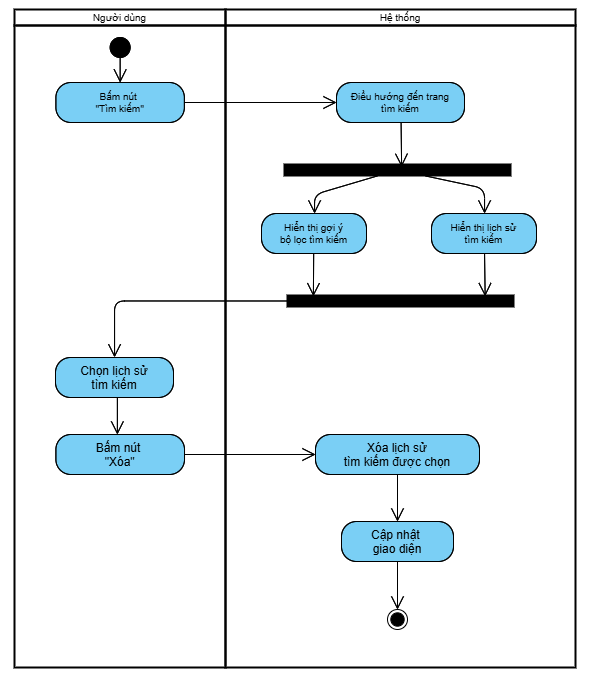
\includegraphics[width=0.6\linewidth]{figures/c3/3-3-17-activity-diagram.png} 
    &  
    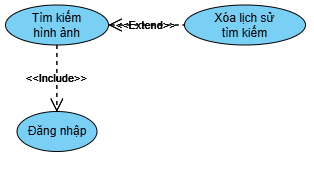
\includegraphics[width=0.35\linewidth]{figures/c3/3-3-17-relationship.png} \\ 
    \hline
\end{tabular}

\begin{figure}[H]
    \centering  
    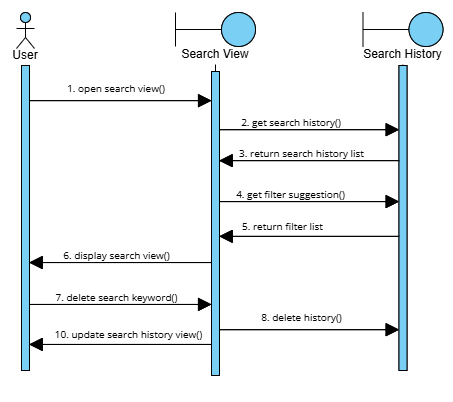
\includegraphics[width=1\textwidth]{figures/c3/3-3-17-sequence-diagram.png}
    \caption{Biểu đồ tuần tự ca sử dụng xóa lịch sử tìm kiếm.}
    \label{fig:3-3-17-sequence-diagram}
\end{figure}